\documentclass{standalone}
\usepackage{tikz}
\usetikzlibrary{patterns, positioning}
\usepackage[sfdefault]{ClearSans} %% option 'sfdefault' activates Clear Sans as the default text font
\usepackage[T1]{fontenc}

\begin{document}
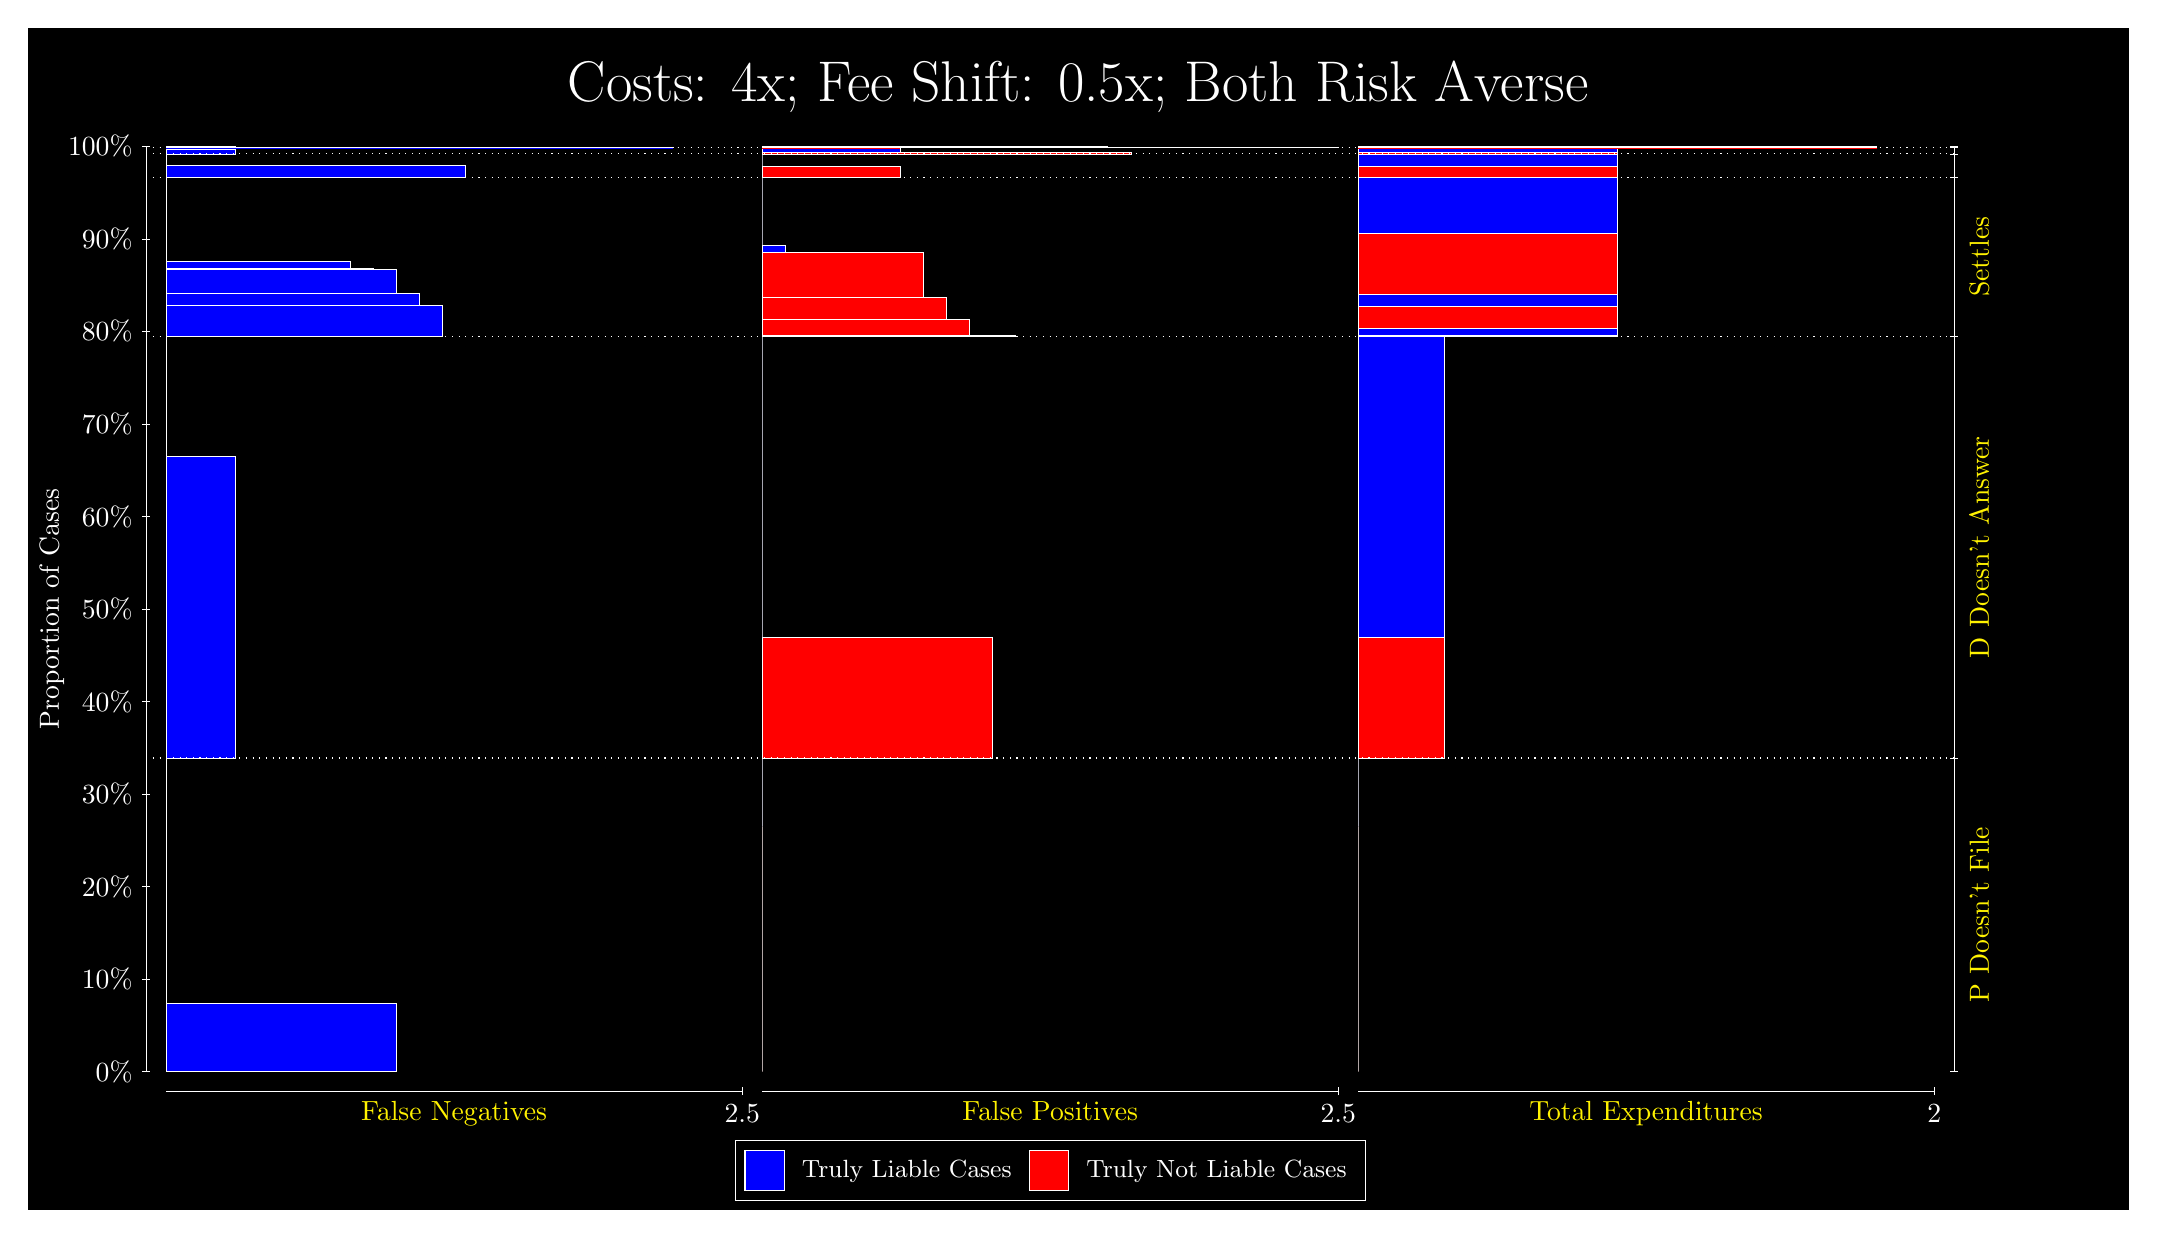
\begin{tikzpicture}
\draw[fill=black] (0,0) rectangle (26.667,15);
\draw[text=white] (0,13.5) rectangle (26.667,15) node[midway] {\huge Costs: 4x; Fee Shift: 0.5x; Both Risk Averse};
\draw[white, very thin] (1.5,1.75) -- (1.5,13.5);
\node[rotate=90, text=white, anchor=center] at (0.3, 7.625) {Proportion of Cases};
\draw[white, very thin] (1.45,1.75) -- (1.55,1.75);
\node[text=white, anchor=east] at (1.45, 1.75) {0\%};
\draw[white, very thin] (1.45,2.925) -- (1.55,2.925);
\node[text=white, anchor=east] at (1.45, 2.925) {10\%};
\draw[white, very thin] (1.45,4.1) -- (1.55,4.1);
\node[text=white, anchor=east] at (1.45, 4.1) {20\%};
\draw[white, very thin] (1.45,5.275) -- (1.55,5.275);
\node[text=white, anchor=east] at (1.45, 5.275) {30\%};
\draw[white, very thin] (1.45,6.45) -- (1.55,6.45);
\node[text=white, anchor=east] at (1.45, 6.45) {40\%};
\draw[white, very thin] (1.45,7.625) -- (1.55,7.625);
\node[text=white, anchor=east] at (1.45, 7.625) {50\%};
\draw[white, very thin] (1.45,8.8) -- (1.55,8.8);
\node[text=white, anchor=east] at (1.45, 8.8) {60\%};
\draw[white, very thin] (1.45,9.975) -- (1.55,9.975);
\node[text=white, anchor=east] at (1.45, 9.975) {70\%};
\draw[white, very thin] (1.45,11.15) -- (1.55,11.15);
\node[text=white, anchor=east] at (1.45, 11.15) {80\%};
\draw[white, very thin] (1.45,12.325) -- (1.55,12.325);
\node[text=white, anchor=east] at (1.45, 12.325) {90\%};
\draw[white, very thin] (1.45,13.5) -- (1.55,13.5);
\node[text=white, anchor=east] at (1.45, 13.5) {100\%};

\draw[white, very thin] (24.457,1.75) -- (24.457,13.5);
\draw[white, very thin] (24.407,1.75) -- (24.507,1.75);
\node[anchor=west] at (24.407, 1.75) {};
\draw[white, very thin] (24.407,5.7318) -- (24.507,5.7318);
\node[anchor=west] at (24.407, 5.7318) {};
\draw[white, very thin] (24.407,11.088) -- (24.507,11.088);
\node[anchor=west] at (24.407, 11.088) {};
\draw[white, very thin] (24.407,13.108) -- (24.507,13.108);
\node[anchor=west] at (24.407, 13.108) {};
\draw[white, very thin] (24.407,13.405) -- (24.507,13.405);
\node[anchor=west] at (24.407, 13.405) {};
\draw[white, very thin] (24.407,13.482) -- (24.507,13.482);
\node[anchor=west] at (24.407, 13.482) {};
\draw[white, very thin] (24.407,13.487) -- (24.507,13.487);
\node[anchor=west] at (24.407, 13.487) {};
\draw[white, very thin] (24.407,13.5) -- (24.507,13.5);
\node[anchor=west] at (24.407, 13.5) {};

\draw[white, very thin, fill=blue] (1.75,1.75) rectangle (4.6775,2.6171);
\draw[white, very thin, fill=red] (1.75,2.6171) rectangle (1.75,5.7318);
\draw[white, very thin, fill=blue] (1.75,5.7318) rectangle (2.6283,9.5581);
\draw[white, very thin, fill=red] (1.75,9.5581) rectangle (1.75,11.088);
\draw[white, very thin, fill=blue] (1.75,11.088) rectangle (5.2631,11.479);
\draw[white, very thin, fill=blue] (1.75,11.479) rectangle (4.9703,11.629);
\draw[white, very thin, fill=blue] (1.75,11.629) rectangle (4.6775,11.944);
\draw[white, very thin, fill=blue] (1.75,11.944) rectangle (4.3848,11.948);
\draw[white, very thin, fill=blue] (1.75,11.948) rectangle (4.092,12.039);
\draw[white, very thin, fill=red] (1.75,12.039) rectangle (1.75,13.108);
\draw[white, very thin, fill=blue] (1.75,13.108) rectangle (5.5558,13.265);
\draw[white, very thin, fill=red] (1.75,13.265) rectangle (1.75,13.405);
\draw[white, very thin, fill=blue] (1.75,13.405) rectangle (2.6283,13.465);
\draw[white, very thin, fill=red] (1.75,13.465) rectangle (1.75,13.482);
\draw[white, very thin, fill=blue] (1.75,13.482) rectangle (8.1906,13.485);
\draw[white, very thin, fill=red] (1.75,13.485) rectangle (1.75,13.487);
\draw[white, very thin, fill=blue] (1.75,13.487) rectangle (2.6283,13.497);
\draw[white, very thin, fill=red] (1.75,13.497) rectangle (1.75,13.5);
\draw[white, very thin, fill=red] (9.3189,1.75) rectangle (9.3189,4.8647);
\draw[white, very thin, fill=blue] (9.3189,4.8647) rectangle (9.3189,5.7318);
\draw[white, very thin, fill=red] (9.3189,5.7318) rectangle (12.246,7.2613);
\draw[white, very thin, fill=blue] (9.3189,7.2613) rectangle (9.3189,11.088);
\draw[white, very thin, fill=red] (9.3189,11.088) rectangle (12.539,11.099);
\draw[white, very thin, fill=red] (9.3189,11.099) rectangle (12.246,11.1);
\draw[white, very thin, fill=red] (9.3189,11.1) rectangle (11.954,11.301);
\draw[white, very thin, fill=red] (9.3189,11.301) rectangle (11.661,11.577);
\draw[white, very thin, fill=red] (9.3189,11.577) rectangle (11.368,12.156);
\draw[white, very thin, fill=blue] (9.3189,12.156) rectangle (9.6116,12.247);
\draw[white, very thin, fill=blue] (9.3189,12.247) rectangle (9.3189,13.108);
\draw[white, very thin, fill=red] (9.3189,13.108) rectangle (11.075,13.248);
\draw[white, very thin, fill=blue] (9.3189,13.248) rectangle (9.3189,13.405);
\draw[white, very thin, fill=red] (9.3189,13.405) rectangle (14.003,13.422);
\draw[white, very thin, fill=blue] (9.3189,13.422) rectangle (11.075,13.482);
\draw[white, very thin, fill=red] (9.3189,13.482) rectangle (11.075,13.485);
\draw[white, very thin, fill=blue] (9.3189,13.485) rectangle (9.3189,13.487);
\draw[white, very thin, fill=red] (9.3189,13.487) rectangle (16.638,13.49);
\draw[white, very thin, fill=blue] (9.3189,13.49) rectangle (13.71,13.5);
\draw[white, very thin, fill=red] (16.888,1.75) rectangle (16.888,4.8647);
\draw[white, very thin, fill=blue] (16.888,4.8647) rectangle (16.888,5.7318);
\draw[white, very thin, fill=red] (16.888,5.7318) rectangle (17.986,7.2613);
\draw[white, very thin, fill=blue] (16.888,7.2613) rectangle (17.986,11.088);
\draw[white, very thin, fill=red] (16.888,11.088) rectangle (20.181,11.099);
\draw[white, very thin, fill=blue] (16.888,11.099) rectangle (20.181,11.19);
\draw[white, very thin, fill=red] (16.888,11.19) rectangle (20.181,11.466);
\draw[white, very thin, fill=blue] (16.888,11.466) rectangle (20.181,11.616);
\draw[white, very thin, fill=red] (16.888,11.616) rectangle (20.181,12.397);
\draw[white, very thin, fill=blue] (16.888,12.397) rectangle (20.181,13.108);
\draw[white, very thin, fill=red] (16.888,13.108) rectangle (20.181,13.248);
\draw[white, very thin, fill=blue] (16.888,13.248) rectangle (20.181,13.405);
\draw[white, very thin, fill=red] (16.888,13.405) rectangle (20.181,13.422);
\draw[white, very thin, fill=blue] (16.888,13.422) rectangle (20.181,13.482);
\draw[white, very thin, fill=red] (16.888,13.482) rectangle (23.475,13.485);
\draw[white, very thin, fill=blue] (16.888,13.485) rectangle (23.475,13.487);
\draw[white, very thin, fill=red] (16.888,13.487) rectangle (23.475,13.49);
\draw[white, very thin, fill=blue] (16.888,13.49) rectangle (23.475,13.5);
\draw[white, dotted] (1.5,5.7318) -- (24.457,5.7318);
\draw[white, dotted] (1.5,11.088) -- (24.457,11.088);
\draw[white, dotted] (1.5,13.108) -- (24.457,13.108);
\draw[white, dotted] (1.5,13.405) -- (24.457,13.405);
\draw[white, dotted] (1.5,13.482) -- (24.457,13.482);
\draw[white, dotted] (1.5,13.487) -- (24.457,13.487);
\draw[white, very thin] (1.75,1.5) -- (9.0689,1.5);
\node[text=yellow, anchor=north] at (5.4094, 1.5) {False Negatives};
\draw[white, very thin] (9.0689,1.45) -- (9.0689,1.55);
\node[text=white, anchor=north] at (9.0689, 1.45) {2.5};

\draw[white, very thin] (9.3189,1.5) -- (16.638,1.5);
\node[text=yellow, anchor=north] at (12.978, 1.5) {False Positives};
\draw[white, very thin] (16.638,1.45) -- (16.638,1.55);
\node[text=white, anchor=north] at (16.638, 1.45) {2.5};

\draw[white, very thin] (16.888,1.5) -- (24.207,1.5);
\node[text=yellow, anchor=north] at (20.547, 1.5) {Total Expenditures};
\draw[white, very thin] (24.207,1.45) -- (24.207,1.55);
\node[text=white, anchor=north] at (24.207, 1.45) {2};

\node[text=yellow, centered, rotate=90] at (24.777, 3.7409) {P Doesn't File};
\node[text=yellow, centered, rotate=90] at (24.777, 8.4097) {D Doesn't Answer};
\node[text=yellow, centered, rotate=90] at (24.777, 12.098) {Settles};





\draw (12.978300999999998,1.5) node[draw=none] (baseCoordinate) {};
\begin{scope}[align=center]
        \matrix[scale=0.5, draw=white, below=0.5cm of baseCoordinate, nodes={draw}, column sep=0.1cm]{
            \node[rectangle, draw, minimum width=0.5cm, minimum height=0.5cm, fill=blue] {}; &
            \node[draw=none, font=\small, text=white] (B) {Truly Liable Cases}; &
            \node[rectangle, draw, minimum width=0.5cm, minimum height=0.5cm, fill=red] {}; &
            \node[draw=none, font=\small, text=white] (B) {Truly Not Liable Cases}; \\
            };
\end{scope}

\end{tikzpicture}
\end{document}